\documentclass[12pt]{article}
\usepackage[utf8]{inputenc}
\usepackage[T1]{fontenc}
\usepackage[spanish, es-noshorthands,activeacute]{babel}
\usepackage[pdftex,usenames,dvipsnames]{color}
%\usepackage{amsmath}
%\usepackage{amssymb}
%\usepackage{mathpazo}
%\usepackage{color}
\usepackage{fancyhdr}
\usepackage{graphicx}
\graphicspath{ {./ImgsPr2/} }
\usepackage{wrapfig}
%\usepackage[shortlabels]{enumitem}
%\usepackage{bm}
%\usepackage{lastpage}
%\usepackage{enumitem}
\usepackage{subcaption}
\usepackage{graphicx}
\DeclareCaptionFormat{custom}
{%
    \textbf{#1#2}\textit{\small #3}
}
\captionsetup{format=custom, labelformat=empty}


\parindent=0mm
\renewcommand*{\baselinestretch}{1.1}
\parskip=5mm
\voffset=-10.4mm
\hoffset=-10.4mm
\oddsidemargin=0mm
\topmargin=0mm
\headheight=4.579965mm
\headsep=3.420035mm
\textwidth=180mm
\textheight=251mm
\marginparsep=0mm
\marginparwidth=0mm
\footskip=8mm
\paperwidth=210mm
\paperheight=297mm

\newcounter{exercise}[section]
\newenvironment{exercise}[2][]{\refstepcounter{exercise}\par\medskip
\noindent \textbf{Exercise~\theexercise.  #2\newline} \rmfamily}{\medskip}

\newenvironment{exercise*}[2][]{\refstepcounter{exercise}\par\medskip
\noindent \textbf{Exercise~\theexercise.  #2\newline} \rmfamily}{\medskip}

\newenvironment{ejercicio}[2][]{\refstepcounter{exercise}\par\medskip
\noindent \textbf{Ejercicio~\theexercise.  #2\newline} \rmfamily}{\medskip}

\newenvironment{apartado}[2][]{\refstepcounter{exercise}\par\medskip
\noindent \textbf{Apartado~\theexercise.  #2\newline} }{\medskip}

\newenvironment{inlinedefinition}[2]
    {\begin{center}
    \begin{tabular}{p{0.9\textwidth}}
    
    \textit{\textbf{#1}.}
    }
    { 
    
    \end{tabular} 
    \end{center}
    }

\pagestyle{fancy}
\fancyhf{}
\lhead{\footnotesize{Teoría de Autómatas y Lenguajes Formales}}
\rhead{\footnotesize{Práctica II}}
\lfoot{\footnotesize{Carlos Martínez Zurita}}
\rfoot{\footnotesize{\thepage}}
\renewcommand{\footrulewidth}{1pt}
\renewcommand{\headrulewidth}{1pt}
\begin{document}
   	\begin{apartado}{Describe el autómata que se pide en el apartado 1 como en el ejemplo 4.1.1 de \textit{talflecturenotes}}
   	El apartado 1 nos pide diseñar un autómata que solo reconozca la cadena $a$. Para evitar que reconozca la cadena vacía, deberá tener al menos dos estados: uno inicial y otro final. Además, para evitar que otras cadenas aparte de $a$ vayan al estado final, habrá un tercer estado foso, y este será en AFD mínimo que cumpla los requisitos (la demostración es trivial, se puede hacer incluso por fuerza bruta, viendo que ningún AFD de dos estados cumple lo que se pide\footnote{Ningún autómata que tenga definidas transiciones con todos los estados y todas las entradas, si no, se podrian eliminar todas las transiciones salvo $(q_0,a,q_1)$}). El autómata obtenido es el siguiente:
   	$\newline K=\{q_0, q_1, q_2\}\newline\Sigma=\{a,b\}\newline\delta=\{(q_0,a,q_1),(q_0,b,q_2),(q_1,a,q_2),(q_1,b,q_2),(q_2,a,q_2),\newline(q_2,b,q_2)\}\newline s=q_0\newline F=\{q_1\}\newline$
   	En la imagen se incluye el resultado de introducir distintas cadenas al autómata, para poder comprobar que solo acepta la cadena $a$.
	\end{apartado}
	\begin{apartado}{Haz el autómata en JFLAP y adjuntar imagen del mismo}
	\begin{figure}[h]
	\centering
	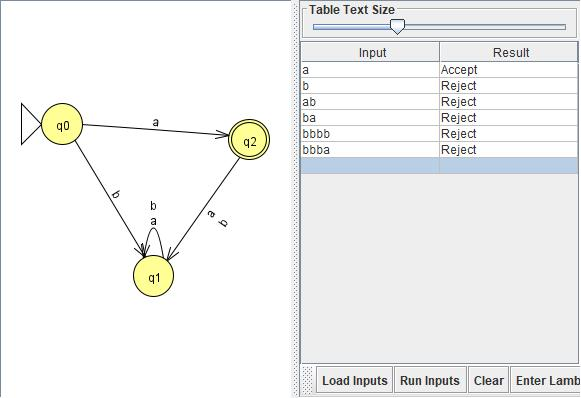
\includegraphics[width=0.4\textwidth]{ej1}
	\caption{Representación del autómata, junto con algunas pruebas}
	\label{fig:figure1}
	\end{figure}
	\end{apartado}
	\begin{apartado}{Describe el autómata en un archivo JSON y cópialo aquí usando el entorno \textit{verbatim}}
	Se ha descrito el autómata de forma que pueda ser reconocido por \textit{finiteautomata.m}, que se encuentra en el repositorio de la asignatura\newpage
		\begin{verbatim}
{
	"name" : "a",
    "representation" : {
      "K" : ["q0", "q1", "q2"],
      "A" : ["a", "b"],
      "s" : "q0",
      "F" : ["q1"],
      "t" : [["q0", "a", "q1"],
             ["q0", "b", "q2"],
             ["q1", "a", "q2"],
             ["q1", "b", "q2"],
             ["q2", "a", "q2"],
             ["q2", "b", "q2"]]
    }
}
		\end{verbatim}
	\end{apartado}
\end{document}